This test problem simulates an incident flux at a shallow angle to
the bottom edge of a 2-D void region.
This test reveals the diffusivity of a transport scheme in the transverse
direction; artificial diffusion will cause the ``sides'' of a radiation beam,
not just the front, to diffuse.
Table \ref{tab:glance_in_void} summarizes the problem parameters.

%-------------------------------------------------------------------------------
\begin{table}[htb]\caption{Glance-in-Void Test Problem Summary}
\label{tab:glance_in_void}
\centering
\begin{tabular}{l l}\toprule
\emph{Parameter} & \emph{Value}\\\midrule
Domain & $\mathcal{D} = (0,10)^2$\\
Initial Conditions & $u_0(\x)=0$\\
Boundary Conditions & $u(\x,t)=\left\{\begin{array}{c c}
  \frac{\pi}{3} & y = 0, \, t > 0\\
  0             & x = 0, \, t > 0
  \end{array}\right. \eqc$\\
Direction & $\di = (0.868890300722,0.350021174582)$,\\
          & normalized such that $\|\di\| = 1$\\
Cross Section & $\sigma(\x)=0$\\
Source & $q(\x,t)=0$\\
Speed & $\speed=1$\\
\bottomrule\end{tabular}
\end{table}
%-------------------------------------------------------------------------------

This test problem was run on a 64$\times$64-cell mesh.
The run parameters are summarized in Table \ref{tab:glance_in_void_run_parameters}.

%-------------------------------------------------------------------------------
\begin{table}[ht]\caption{Normal Void-to-Absorber Test Problem Run Parameters}
\label{tab:glance_in_void_run_parameters}
\centering
\begin{tabular}{l l}\toprule
\emph{Parameter} & \emph{Value}\\\midrule
Number of Cells & $N_{cell} = 4096$\\
Time Discretization & Explicit Euler, SSPRK33\\
End Time & $t = 2$\\
CFL Number & $\nu = 0.5$\\\midrule
Entropy Function & $\entropy(\scalarsolution) = \frac{1}{2}\scalarsolution^2$\\
Entropy Residual Coefficient & $\entropyresidualcoef = 0.1, 0.5, 1.0$\\
Entropy Jump Coefficient & $\entropyjumpcoef = 0.1, 0.5, 1.0$\\\midrule
FCT Solution Bounds & DMP\\
\bottomrule\end{tabular}
\end{table}
%-------------------------------------------------------------------------------
\begin{figure}[ht]
   \centering
   \begin{subfigure}{0.45\textwidth}
      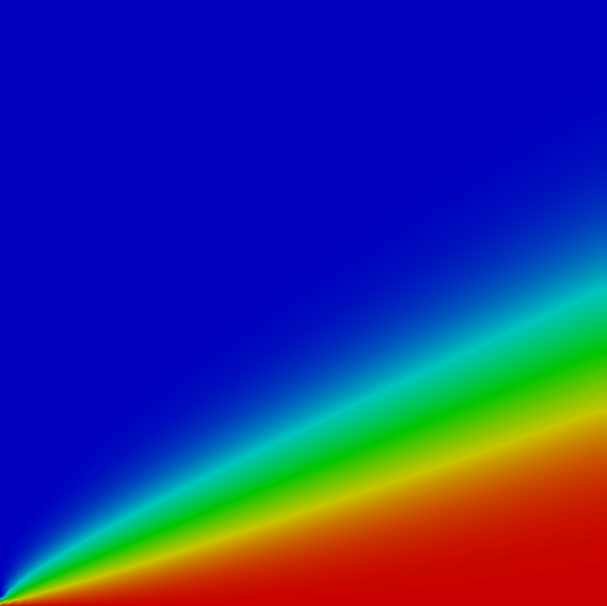
\includegraphics[width=\textwidth]
        {\contentdir/results/transport/glance_in_void/images/DMP_FE.png}
      \caption{Low-Order}
   \end{subfigure}
   \begin{subfigure}{0.45\textwidth}
      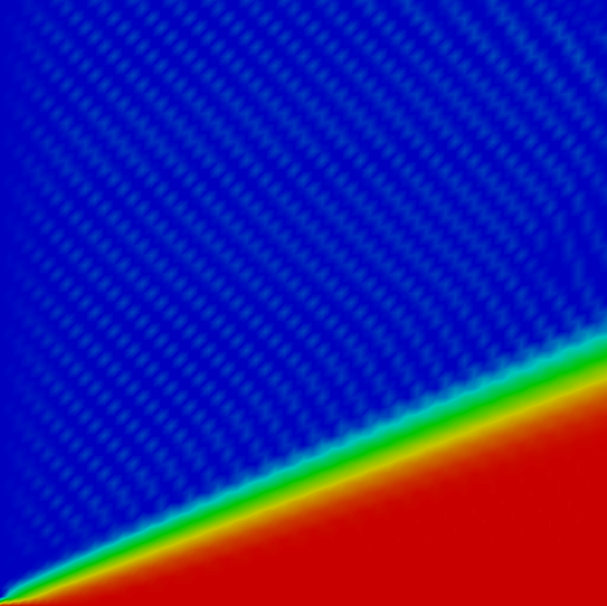
\includegraphics[width=\textwidth]
        {\contentdir/results/transport/glance_in_void/images/EV_FE_cE1.png}
      \caption{EV, $\entropyresidualcoef=1.0$}
   \end{subfigure}
   \begin{subfigure}{0.45\textwidth}
      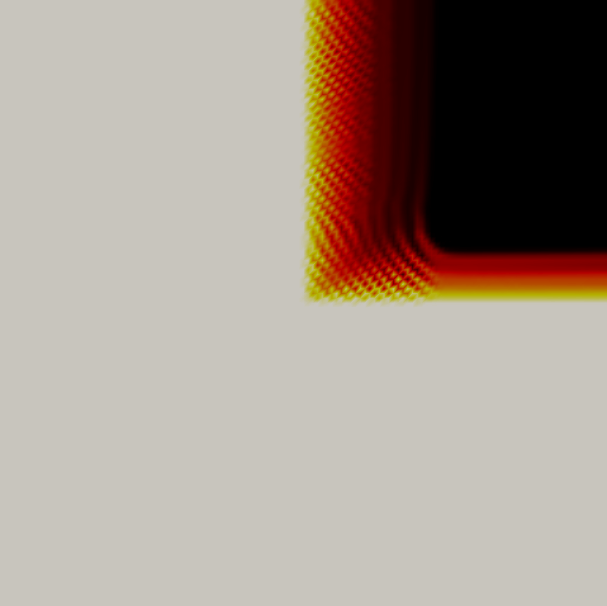
\includegraphics[width=\textwidth]
        {\contentdir/results/transport/glance_in_void/images/GalFCT_FE.png}
      \caption{Galerkin-FCT}
   \end{subfigure}
   \begin{subfigure}{0.45\textwidth}
      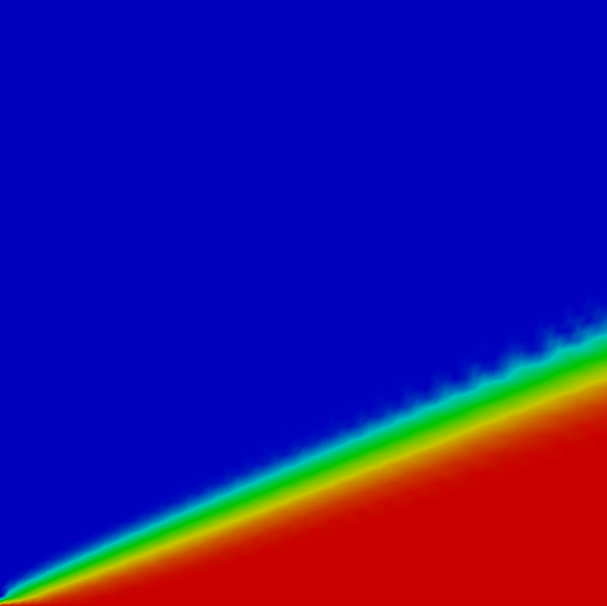
\includegraphics[width=\textwidth]
        {\contentdir/results/transport/glance_in_void/images/EVFCT_FE_cE1.png}
      \caption{EV-FCT, $\entropyresidualcoef=1.0$}
   \end{subfigure}
   \caption{Comparison of Solutions for the Glance-in-Void Test
     Problem Using Explicit Euler Time Discretization with 4096 Cells}
   \label{fig:glance_in_void_fe}
\end{figure}
%-------------------------------------------------------------------------------
\begin{figure}[ht]
   \centering
   \begin{subfigure}{0.3\textwidth}
      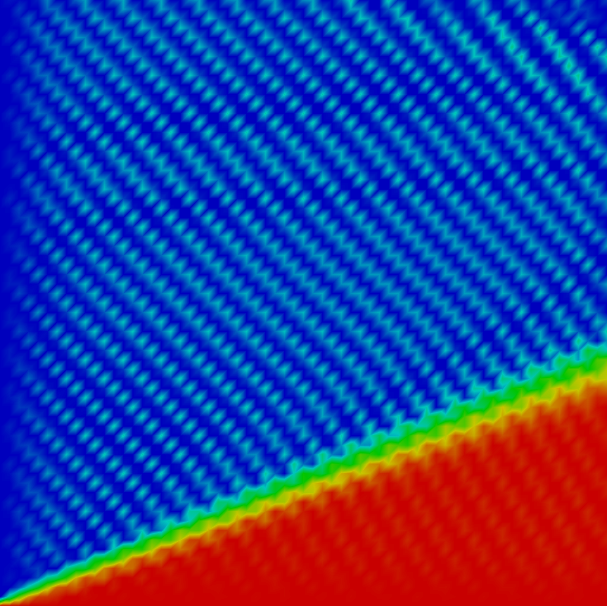
\includegraphics[width=\textwidth]
        {\contentdir/results/transport/glance_in_void/images/EV_FE_cE01.png}
      \caption{EV, $\entropyresidualcoef=0.1$}
   \end{subfigure}
   \begin{subfigure}{0.3\textwidth}
      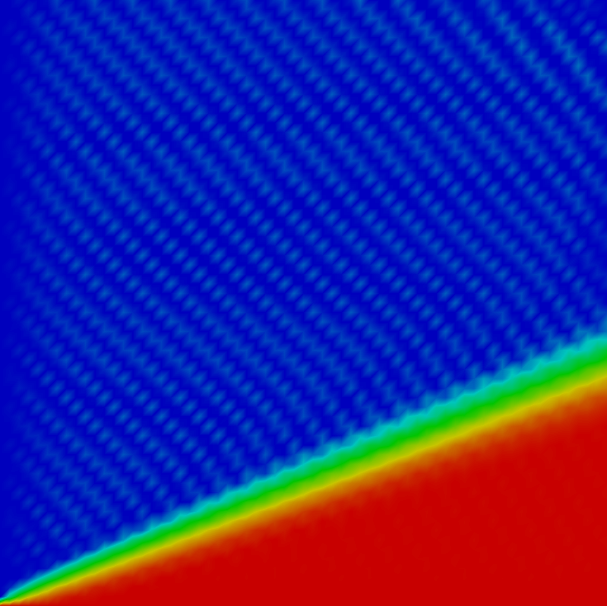
\includegraphics[width=\textwidth]
        {\contentdir/results/transport/glance_in_void/images/EV_FE_cE05.png}
      \caption{EV, $\entropyresidualcoef=0.5$}
   \end{subfigure}
   \begin{subfigure}{0.3\textwidth}
      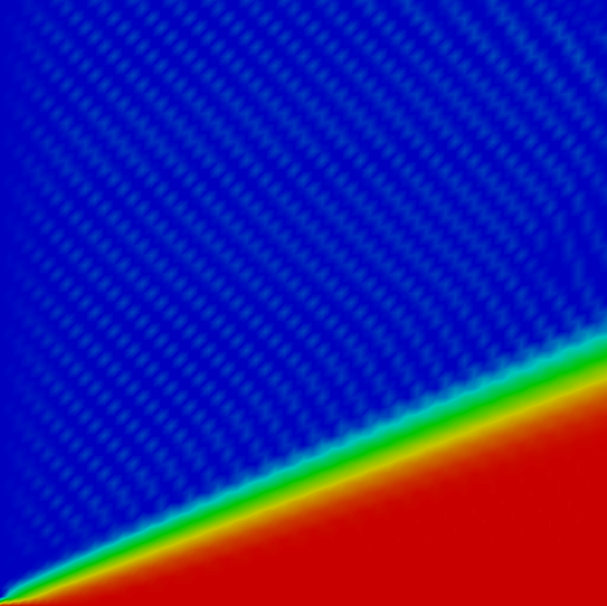
\includegraphics[width=\textwidth]
        {\contentdir/results/transport/glance_in_void/images/EV_FE_cE1.png}
      \caption{EV, $\entropyresidualcoef=1.0$}
   \end{subfigure}
   \begin{subfigure}{0.3\textwidth}
      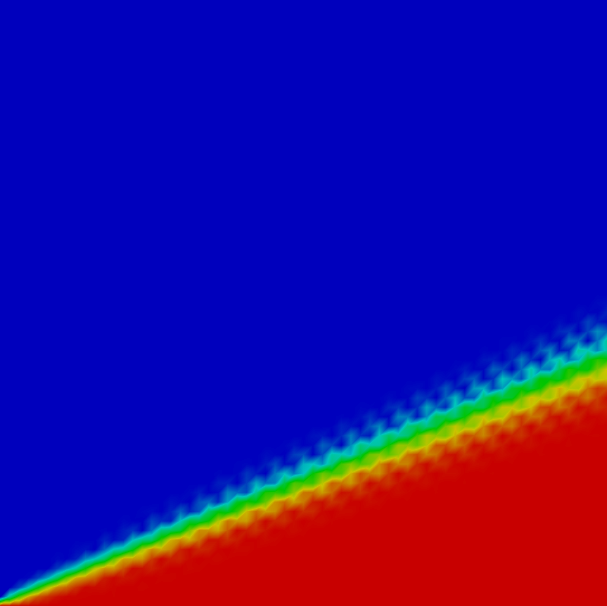
\includegraphics[width=\textwidth]
        {\contentdir/results/transport/glance_in_void/images/EVFCT_FE_cE01.png}
      \caption{EV-FCT, $\entropyresidualcoef=0.1$}
   \end{subfigure}
   \begin{subfigure}{0.3\textwidth}
      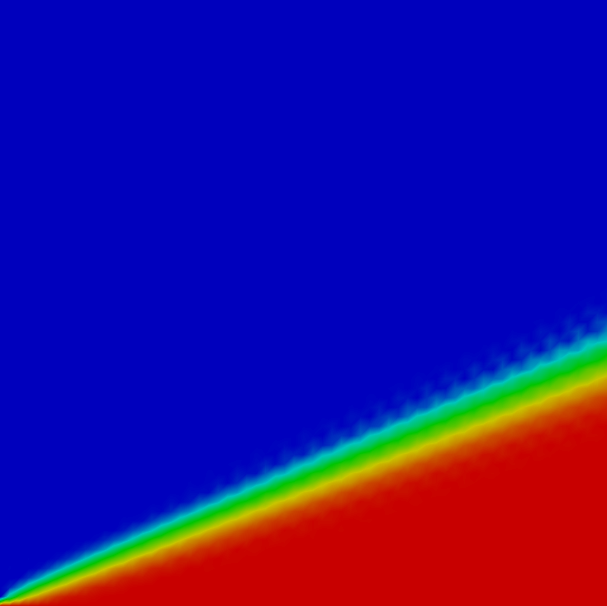
\includegraphics[width=\textwidth]
        {\contentdir/results/transport/glance_in_void/images/EVFCT_FE_cE05.png}
      \caption{EV-FCT, $\entropyresidualcoef=0.5$}
   \end{subfigure}
   \begin{subfigure}{0.3\textwidth}
      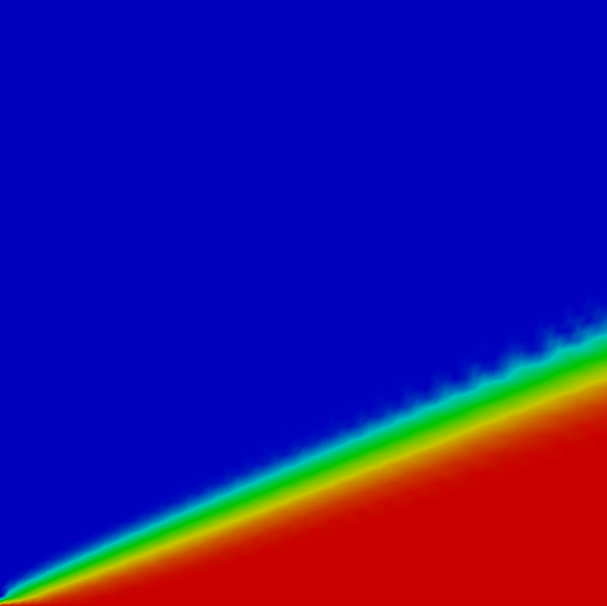
\includegraphics[width=\textwidth]
        {\contentdir/results/transport/glance_in_void/images/EVFCT_FE_cE1.png}
      \caption{EV-FCT, $\entropyresidualcoef=1.0$}
   \end{subfigure}
   \caption{Comparison of EV and EV-FCT Solutions for the Glance-in-Void Test
     Problem Using Explicit Euler Time Discretization with 4096 Cells
     and Various $\entropyresidualcoef$ Values}
   \label{fig:glance_in_void_fe_cE}
\end{figure}
%-------------------------------------------------------------------------------
\begin{figure}[ht]
   \centering
   \begin{subfigure}{0.45\textwidth}
      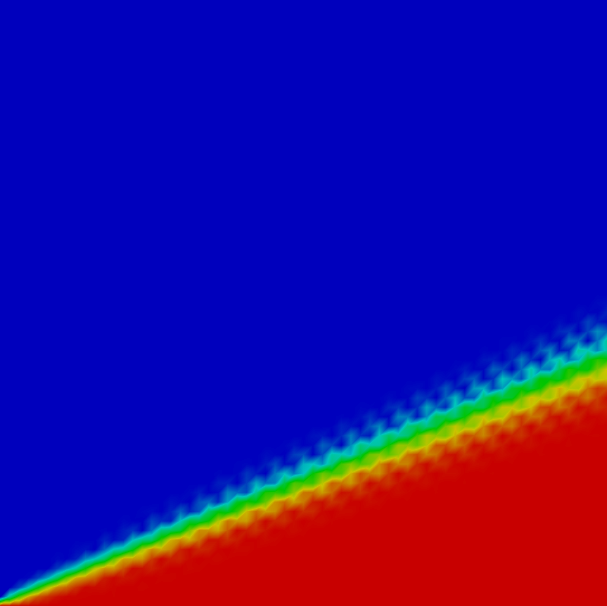
\includegraphics[width=\textwidth]
        {\contentdir/results/transport/glance_in_void/images/EVFCT_FE_cE01.png}
      \caption{EV-FCT, FE, $\entropyresidualcoef=0.1$}
   \end{subfigure}
   \begin{subfigure}{0.45\textwidth}
      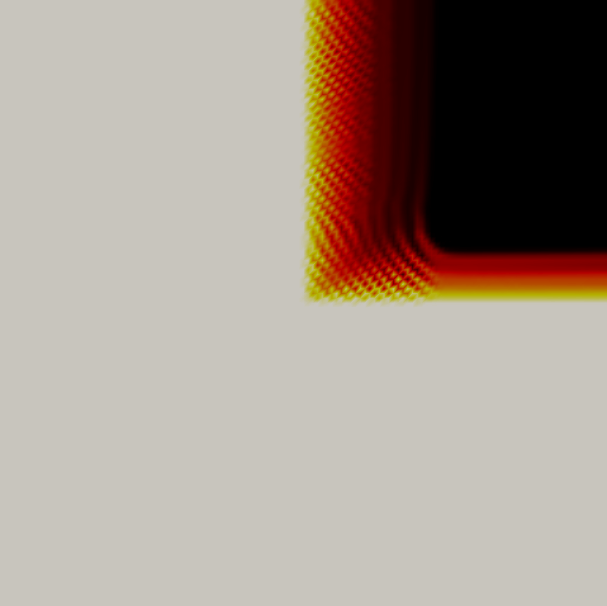
\includegraphics[width=\textwidth]
        {\contentdir/results/transport/glance_in_void/images/GalFCT_FE.png}
      \caption{Galerkin-FCT, FE}
   \end{subfigure}
   \begin{subfigure}{0.45\textwidth}
      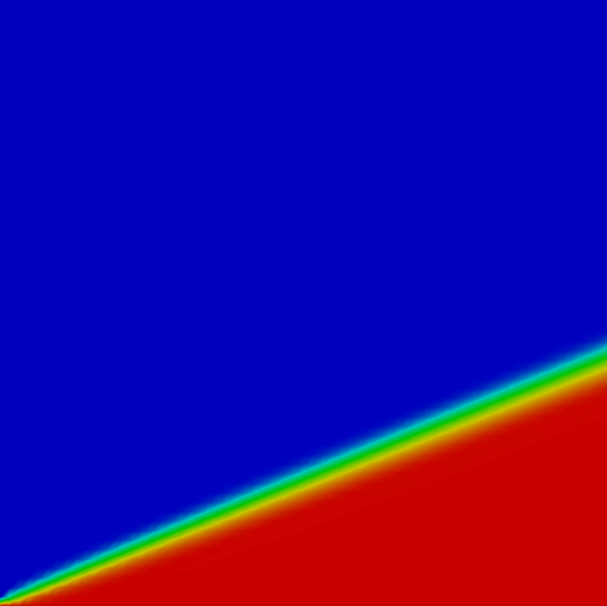
\includegraphics[width=\textwidth]
        {\contentdir/results/transport/glance_in_void/images/EVFCT_SSP3_cE01.png}
      \caption{EV-FCT, SSPRK33, $\entropyresidualcoef=0.1$}
   \end{subfigure}
   \begin{subfigure}{0.45\textwidth}
      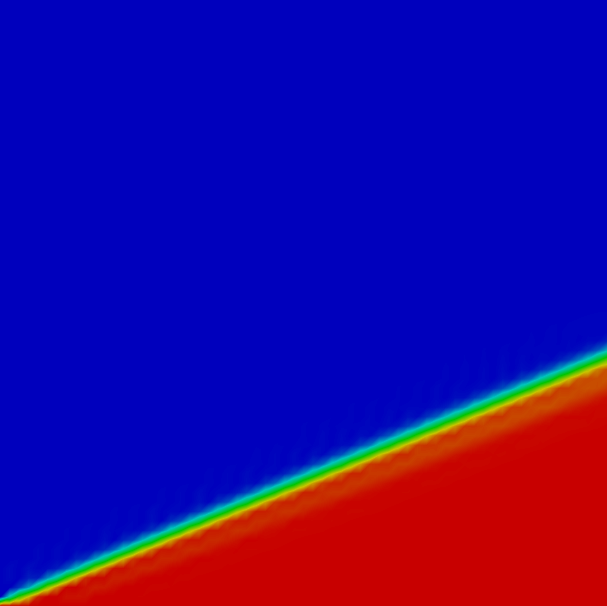
\includegraphics[width=\textwidth]
        {\contentdir/results/transport/glance_in_void/images/GalFCT_SSP3.png}
      \caption{Galerkin-FCT, SSPRK33}
   \end{subfigure}
   \caption{Comparison of Solutions for the Glance-in-Void Test
     Problem Using Explicit Euler vs. SSPRK33 with 4096 Cells}
   \label{fig:glance_in_void_fe_vs_ssprk}
\end{figure}
%-------------------------------------------------------------------------------

\clearpage

